\chapter{Смешение волн на $\Delta$-системе}
Как упоминалось ранее, долгое время исследования в экспериментальной квантовой оптике были сосредоточены на изучении ансамблей природных, или естественных атомов \cite{Miller_2005,Walther_2006}. Однако, сверхпроводящие искусственные атомы крайне привлекательны для изучения явлений квантовой оптики. Их энергетические уровни могут быть спроектированы со значительным отличием от естественных атомов, и сильная связь с полем достигается не только в высокодобротных резонаторах \cite{wallraff2004strong}, но и в линих передачи (волноводах) \cite{Astafiev2010resonance, vanLoo1494}. Это позволяет воспроизводить явления квантовой оптики и даже достигать режимов, недоступных для естественных атомов. Интерес для применений представляют такие явления, как когерентный захват заселенности, электромагнитно-индуцированная прозрачность, расщепление Аутлера-Таунса --- многие из них были представлены в разделе \ref{sec: microwave qo}. В данной работе представлены также результаты по непрерывному волновому смешению (Глава \ref{ch: cwm}) и квантовому волновому смешению (Глава \ref{ch: q_mixing}), которые были впервые экспериментально изучены в сверхпроводящих искусственных атомах. Кроме того, сверхпроводящие трехуровневые системы могут быть использованы для охлаждения квантовых систем, усиления микроволновых сигналов и генерации одиночных или запутанных пар фотонов --- всего того, что является важным для создания квантовых сетей \cite{kimble2008quantum}.

В данной главе представлены результаты эксперимента по трехволновому квантовому смешению \cite{liu2014controllable}. Это нелинейный эффект, который может возникать в циклических трехуровневых атомах, фактически отсутствующих в природе, но легко реализуемых с помощью сверхпроводящих искусственных атомов. Единственными подходящими естественными системами для трехволнового смешения являются хиральные молекулярные трехуровневые системы без инверсионной симметрии \cite{PhysRevLett.111.023008}. Однако эти системы не могут быть перестраиваемыми по частоте. В отличие от параметрических трехволновых смесительных устройств на основе джозефсоновского перехода, которые полагаются на смешивание по классической нелинейности, мы реализуем здесь другой метод генерации трехволнового смешивания с использованием одного искусственного атома циклического типа, или $\Delta$-типа. Это явление теоретически рассмотрено в работах. Мы непосредственно измеряем когерентное излучение циклического трехуровневого атома при двух внешних резонансных возбуждающих сигналах, соответствующих двум атомным переходам \cite{PhysRevA.98.041801}. Излучение происходит на одной частоте --- сумме или разности частот драйва. Это излучение является следствием когерентного преобразования частоты, но по своей сути отличается от классического нелинейного преобразования частоты, которое привело бы к появлению боковых компонент на суммарной и разностной частотах. Ранее когерентные атомные возбуждения с использованием двух частот были исследованы при помощи фазового кубита, являющегося квантовой системой с двумя внутренними степенями свободы \cite{Lecocq2012}. Однако, состояние фазового кубита измерялось с помощью тока переключения, в то время как прямое детектирование когерентно преобразованного сигнала на циклическом искусственном атоме в открытом пространстве дает некоторые преимущества. В частности, можно непосредственно использовать когерентную (упругую) составляющую излучаемого поля на суммарной или разностной частоте переходов искусственного атома. Это открывает путь к инновационной квантовой электронике на основе трехволнового смешения или когерентного преобразования частоты.
\section{Режим $\Delta$-системы в потоковом кубите}
\begin{figure}
	\centering
	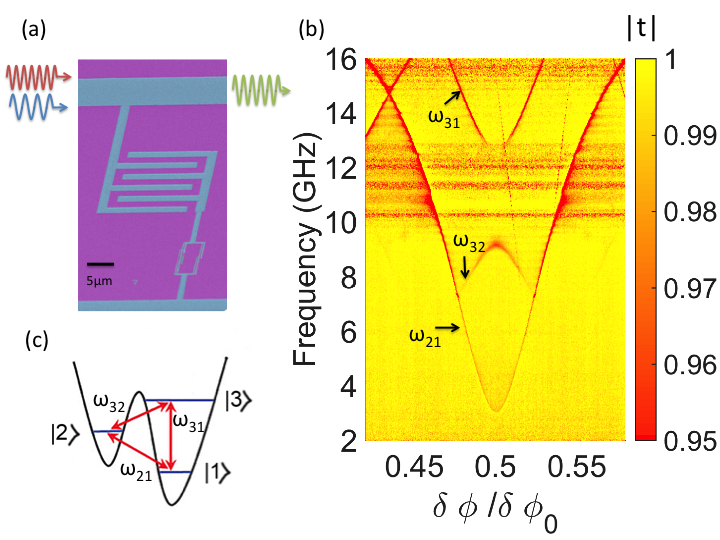
\includegraphics[width=0.8\textwidth]{figure1_Delta.png}
	\caption[Потоковый кубит в режиме $\Delta$-системы]{Сильно связанный с волноводом потоковый кубит, состоящий из 4 джозефсоновских переходов, электронное изображение которого представлено на панели (a), может находиться в режиме $\Delta$-системы при $\delta\phi \ne 0.5$. Однотоновая спектроскопия представлена на графике (b), верхние переходы становятся видимыми из-за большой мощности тона. (с), принципиальная схема переходов в циклическом атоме. Измерения проводятся при $\omega_{21}/2\pi = 6.48$ ГГц, $\omega_{32}/2\pi = 8.35$ ГГц, и $\omega_{31}/2\pi = 14.83$ ГГц.}
	\label{fig: flux_delta}
\end{figure}
Изучаемое устройство представляет собой потоковый кубит --- сверхпроводниковую петлю площадью около $\sim 10$~мкм$^{2}$, в которую вставлены четыре джозефсоновских перехода. Эта геометрия является модифицированной версией оригинального потокового кубита, предложенного в работе \cite{mooij1999josephson}, где один из трех переходов --- $\alpha$-переход --- имеет в $\alpha$ раз отличную площадь по сравнению с остальными переходами. Один из электродов получившейся петли связан с одномерным волноводом через встречно-штыревую емкость $C=6$~фФ, см. Рис.~\ref{fig: flux_delta}(a). resulting into a photon rate in the range from several MHz to a few tens of MHz depending on frequency. Основные параметры устройства --- джозефсоновская энергия $E_{J}/h=65$~ГГц, зарядовая энергия $E_{C}=e^2/2C$, $E_{C}/h=19$~ГГц и параметр $\alpha=0.45$ --- подобраны таким образом, чтобы все три частоты нижних переходов атома, см. Рис.~\ref{fig: flux_delta}c), попадали в допустимый частотный диапазон 2-18 ГГц нашего высокочастотного измерительного тракта. Скорость излучения в волновод для каждого из этих переходов достаточно велика для того, чтобы безызлучательная релаксация не играла значительной роли для наблюдаемых нами явлений. 

Точные значения частот переходов $\omega_{12}$, $\omega_{23}$, и $\omega_{13}$ контролируются при помощи внешнего магнитного потока, пронизывающего петлю кубита, $\Phi=\Phi_{0}/2+\delta\Phi$, где $\Phi_{0}$ --- квант магнитного потока и $\delta\Phi$ --- отстройка по потоку от точки симметрии, которая соответствует половине кванта магнитного потока. Частоты атомных переходов экспериментально определяются при помощи однотоновой спектроскопии на пропускание, измеряемой при помощи ВАЦ. Мы сканируем частоту пробного сигнала при различных значениях $\delta\Phi$, в результате получая спектр на Рис.~\ref{fig: flux_delta}b). Чтобы увидеть переход $|3\rangle \rightleftarrows |2\rangle$, необходимо значительно поднять мощность микроволнового тона, чтобы вызвать заметную заселенность уровня $\ket{2}$, который практически не заселяется в пределе слабой мощности. 
В рабочей точке по магнитному потоку частоты разрешенных переходов составляют $\omega_{21}/2\pi = 6.48$ ГГц, $\omega_{32}/2\pi = 8.35$ ГГц, и $\omega_{31}/2\pi = 14.83$ ГГц ($\omega_{31} = \omega_{21}+\omega_{32}$),  как схематично показано на Рис.~\ref{fig: flux_delta}(c). Отметим, что все три вышеперечисленные перехода разрешены только при ненулевой отстройке от $\delta\Phi = \Phi_0/2$, в то время как в точке симметрии переход $\ket{1}\rightleftarrows\ket{3}$ является запрещенным из соображений симметрии. Все измерения проводятся при базовой температуре криостата 12-15 мК, при которой тепловая заселенность пренебрежимо мала и не оказывает влияния на ход эксперимента.

\section{Описание эксперимента}
После завершения начальной характеризации образца, мы подаем на $\Delta$-систему два непрерывных сигнала, частоты которых практически совпадают с резонансными частотами каких-либо двух атомных переходов, и изучаем когерентное излучение системы на частоте третьего перехода, не возбуждаемого внешними сигналами. 
Измерения в каждом из показанных на Рис.~\ref{fig: 3wm_regimes} режимов проводились при различных значениях амплитуд Раби внешнего поля $\Omega_{ij}$ между состояниями $\ket{i}, \ket{j}$, где $i$ и $j$ принимают значения 1,2,3. Согласно квантовомеханическому описанию, излучение на боковой компоненте может возникнуть только в том случае, если она попадает в резонанс с каким-либо атомным переходом.
\begin{figure}
	\centering
	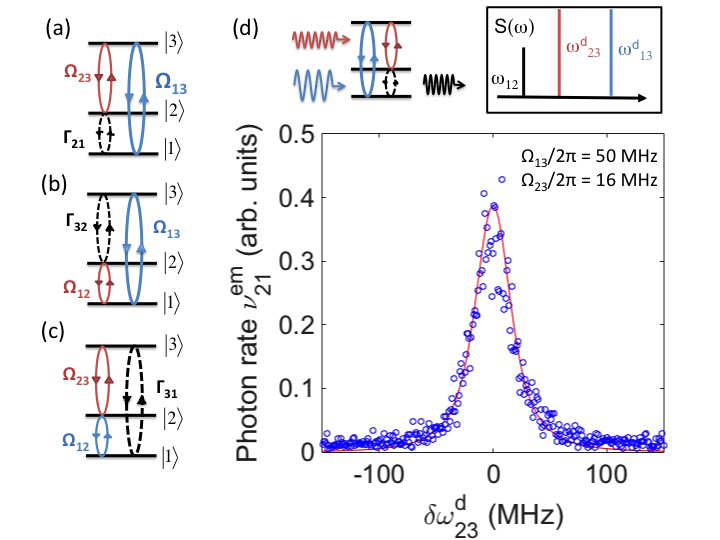
\includegraphics[width=0.8\textwidth]{figure2_Delta.png}
	\caption[Режимы трехволнового смешения на трехуровневой $\Delta$-системе]{Когерентное излучение на трехуровневой системе. Атом накачивается гармоническими сигналами на частотах: (a) $\omega_{23}$ и $\omega_{13}$; (b) $\omega_{12}$ и $\omega_{13}$; (c) $\omega_{12}$ и $\omega_{23}$. Амплитуды полей обозначены как $\Omega$ с индексами, соответствующими номерам уровней. (d) Мощность пика когерентного излучения на частоте $\omega_{12}$ в зависимости от отстройки $\delta\omega_{23}$, выраженная в единицах потока фотонов $\nu_{21}^{\text{em}}$. Атом находится под действием сигналов с амплитудами $\Omega_{23}/2\pi=16$ МГц, $\Omega_{13}/2\pi=50$ МГц, as a function of detuning of the driving frequency, $\delta\omega_{23}^{d}$. Вставка в правом верхнем углу схематично отражает полный спектр излучения $\Delta$-системы. }
	\label{fig: 3wm_regimes}
\end{figure}
Чтобы понять механизм происходящих физических процессов, можно обратиться к формализму вторичного квантования. При взаимодействия двух когерентных волн с одиночной квантовой системой, только один акт рассеяния (однофотонного или многофотонного) может происходить одномоментно, так как испущенное излучение улетает в волновод, и каскадные процессы становятся невозможными. Введем операторы рождения и уничтожения фотона  $a^{\dagger}_{ij} \text{ и }a_{ij}$ на частоте $\omega_{ij}$, тогда разрешенные многофотонные процессы, ограниченные атомными переходами, описываются членами $a_{31}a_{32}^{\dagger}a_{21}^{\dagger}$ и $a_{31}^{\dagger}a_{32}a_{21}$. Эти два процесса сохраняют полную энергию и объясняют создание фотонов на дополнительных частотах, изображенных на Рис.~\ref{fig: 3wm_regimes}(a-c) пунтктирными линиями.

\section{Расчет амплитуды боковой компоненты}
